% If enabled, this produces a notes-free version for handing out
%\def\HANDOUT{}
% If enabled in tandem with \HANDOUT, doesn't reformat the slides to fit on a
% single page
%\def\EMAILEDCOPY{}

\documentclass[
    aspectratio=169,
    \ifdefined\HANDOUT
    handout
    \else
    \fi
]{beamer}
\usetheme{AnnArbor}
\usecolortheme{illini}
\setbeamertemplate{note page}[]
\ifdefined\HANDOUT
\ifdefined\EMAILEDCOPY
\else
\usepackage{pgfpages}
\pgfpagesuselayout{resize to}[letterpaper,border shrink=2mm, landscape]
\fi
\else
%\setbeameroption{show notes}
%\setbeameroption{show notes on second screen=bottom}
\fi
\setbeamertemplate{caption}[numbered]

%TODO Font should be adjusted (bigger)
\usepackage[]{amsfonts}
\newcommand{\overbar}[1]{\mkern 1.5mu\overline{\mkern-1.5mu#1\mkern-1.5mu}\mkern 1.5mu}
\usepackage{amsmath}
\usepackage{amssymb}
\usepackage{mathtools}
\usepackage{listings}
\usepackage{algorithm}
\usepackage{algpseudocode}
\usepackage{ulem}
\usepackage{censor}

%\usepackage{biblatex}
%\renewcommand*{\bibfont}{\small}

\DeclareMathOperator*{\argmax}{arg\,max}
\DeclareMathOperator*{\argmin}{arg\,min}

\graphicspath{img}

\title[ECC 2026]{Data-Driven Control of Inverter-Based Microgrids}
\subtitle{ECC 2026}
\author[TA, ES, TGR, ADG]{Temitope Amuda, Eric Silk, T.G. Roberts, Alejandro Dominguez-Garcia}
\institute[ECE@UIUC]{Electrical and Computer Engineering\linebreak University of Illinois at Urbana-Champaign}
\date{July 9, 2026}
\logo{
\includegraphics[height=1cm]{img/template/small_logo.png}}
\begin{document}
\definecolor{UIUCOrange}{RGB}{255,95,5}
\definecolor{UIUCBlue}{RGB}{19,41,75}
\definecolor{UIUCBlueSubhead}{RGB}{5,86,165}
\definecolor{UIUCBlueKnockoutheader}{RGB}{32,64,151}
\definecolor{UIUCGray1}{RGB}{232,233,234}
\definecolor{UIUCGray2}{RGB}{166,168,171}
\definecolor{UIUCGray3}{RGB}{94,102,105}

\begin{frame}
    \titlepage
    \tiny
    Compiled: \today
\end{frame}

\section{Background}

\subsection*{Motivation}
\begin{frame}
    \frametitle{Motivation}
    \begin{itemize}
        \item Microgrids often use Inverter-Based Resources (IBRs)
        \item System models are often missing or incomplete
        \item \begin{itemize}
                  \item Topology changes
                  \item Controller Gains
              \end{itemize}
        \item Improved telemetry $\implies$ lots of data to work with
    \end{itemize}
\end{frame}

\subsection*{Model-Predictive Control}
\begin{frame}
    \frametitle{Model-Predictive Control}
    \begin{columns}
        \begin{column}[T]{0.5\textwidth}
            \textbf{Uses:}
            \begin{itemize}
                \item Online, recursive estimation
                \item Linearized Model(s)
                \item Succesive operating points
            \end{itemize}
        \end{column}
        \begin{column}[T]{0.5\textwidth}
            \textbf{Doesn't need:}
            \begin{itemize}
                \item System Model
                \item Inverter Types
                \item Inverter Control Gains
            \end{itemize}
        \end{column}
    \end{columns}
\end{frame}
%\begin{frame}[t]
%    \frametitle{Prior Art}
%    \begin{columns}
%        \begin{column}[T]{0.5\textwidth}
%            \vspace{0pt}
%            \begin{center}
%                \textbf{Bulk Systems}
%            \end{center}
%            \begin{itemize}
%                \item Model-free disturbance estimator\cite{Ekomwenrenren2024}
%                \item Data-driven frequency, voltage, tie-line regulation\cite{MadiADG2021}
%                \item Sensitivity-based voltage regulation via online topology identification\cite{Liu2021}
%                \item Online feedback voltage regulation\cite{Domin2023}
%            \end{itemize}
%        \end{column}
%        \begin{column}[T]{0.5\textwidth}
%            \vspace{0pt}
%            \begin{center}
%                \textbf{Microgrids}
%            \end{center}
%            \begin{itemize}
%                \item Adaptive Koopman Operator\cite{Gong2023}
%                \item Distributed Online Neural Network\cite{Zheng2022}
%                \item Adaptive multi-model\cite{Ma2021}
%            \end{itemize}
%        \end{column}
%    \end{columns}
%\end{frame}

\subsection*{Preliminaries}
%\begin{frame}
%    \frametitle{Power Flow}
%    Balanced, three-phase with $N$ buses where $\mathcal{N}=\left\{1,\ldots,N\right\}$.
%    \begin{subequations}\label{pfproblem}
%        \begin{align}
%            P_{i}(t) & = \sum_{j=1}^N V_{i}(t)V_{j}(t)\Big(G_{ij}\cos{\big(\theta_{i}(t)-\theta_{j}(t)\big)} \nonumber
%            +B_{ij}\sin{\big(\theta_{i}(t)-\theta_{j}(t)\big)\Big)},                                                   \\
%            Q_{i}(t) & = \sum_{j=1}^N V_{i}(t)V_{j}(t)\Big(G_{ij}\sin{\big(\theta_{i}(t)-\theta_{j}(t)\big)}\nonumber
%            -B_{ij}\cos{\big(\theta_{i}(t)-\theta_{j}(t)\big)\Big)},\end{align}
%    \end{subequations}
%    where $G_{ij}$ and $B_{ij}$ are the $(i,j)$-th entries of conductance/suseptance matrices
%\end{frame}
%\begin{frame}
%    \frametitle{Dispatchable Virtual Oscillator Control (dVOC) Equations}
%    \begin{align}
%        \omega_{i}(t) = & ~ \omega^\circ+\frac{\omega^\circ\kappa_{1,i}}{V_{i}^2(t)}\big(P_{i}^{\circ}(t)-P_{i}(t)\big), \\
%        \dot{V}_i(t)=   & ~\omega^\circ\kappa_{2,i}\big((V_i^\circ)^2-V_{i}^2(t)\big)V_{i}(t)\nonumber
%        +\frac{\omega^\circ\kappa_{1,i}}{V_{i}(t)}\big(Q_{i}^{\circ}(t)-Q_{i}(t)\big),
%    \end{align}
%    where $V_i^\circ$ is nominal GFM inverter voltage mag, $\kappa_{1,i}$ is sync gain, and $\kappa_{2,i}$ is voltage amplitude gain.
%    \note[item]{}
%    \note[item]{}
%    \note[item]{}
%\end{frame}
\begin{frame}
    \frametitle{Controllability}
    \begin{center}
        Not all IBRs are controllable!
    \end{center}
    \begin{align*}
        P_{i}^{\circ}(t)=\begin{cases} P_{i}^{r}(t), &i=1,2,\ldots, m,\\ P_{i}^{d}(t), &i=m+1,m+2,\ldots, N,\end{cases}
    \end{align*}

    \begin{align*}
        Q_{i}^{\circ}(t)=\begin{cases} Q_{i}^{r}(t), &i=1,2,\ldots, m,\\ Q_{i}^{d}(t), &i=m+1,m+2,\ldots, N,\end{cases}
    \end{align*}
    where the $r$ superscript indicates controllable devices and $d$ indicates
    uncontrollable devices.
    \note[item]{Some IBRs are controllable, some aren't}
    \note[item]{$1..m$ are controllable}
    \note[item]{$m+1..N$ are not controllable}
\end{frame}
\begin{frame}
    \frametitle{Average Frequency Error}
    Let $\omega_i$ be the frequency at bus $i$ and $\omega^0$ is the nominal frequency. Then,
    \begin{align*}
        \overline{\Delta \omega}(t) & := \frac{1}{m}\sum_{i=1}^{m}\omega_i(t)-\omega^{\circ}
    \end{align*}
    is the average frequency error.
    \begin{center}
        \textbf{We want to drive this value to 0, and voltages at the controllable buses to 1 p.u.!}
    \end{center}
    \note[item]{Unweighted average of frequency errors (pretty self-explanatory)}
    \note[item]{Frequency adjusted by active power}
    \note[item]{Voltage adjusted by reactive power}
\end{frame}

\section{Online Estimation}
\subsection*{Linearization of the System}
\begin{frame}
    \frametitle{Problem Formulation}
    Define:
    \begin{align*}
        \theta(t) & = [\theta_1(t), \theta_2(t), \dots,
        \theta_m(t)]^\top,                                                                  \\
        V(t)      & = [V_1(t), V_2(t), \dots, V_m(t)]^\top,                                 \\
        P^r(t)    & = [P_1^r(t),  P_2^r(t), \dots,  P_m^r(t)]^\top,                         \\
        Q^r(t)    & = [Q_1^r(t), Q_2^r(t), \dots,
        Q_m^r(t)]^\top,                                                                     \\
        x(t)      & = [\theta^\top (t), ~V^\top (t)]^\top \in \mathbb{R}^n,                 \\
        u(t)      & = \big[\big(P^r(t))^\top, ~\big(Q^r(t))^\top\big]^\top \in \mathbb{R}^n \\
    \end{align*}
    The dynamics of the controllable buses then:
    \begin{align*}
        \dot{x}(t) & = f\big(x(t),u(t),\xi(t)\big)
    \end{align*}
    where $n=2m$ and $\xi(t)\in \mathbb{R}^l$ denotes unmodeled dynamics/exogenous disturbances.
    \note[item]{the system in \ref{the_system} is a reduced order model}
    \note[item]{$\xi(t)$ is bounded, varies slowly with time, and is uncorrelated with the control input $u(t)$.}
    \note[item]{We can assume the system is bounded-input, bounded-output stable}
\end{frame}
%\begin{frame}
%    \frametitle{Discrete Time}
%    For some sufficiently small $T>0$ and $k=0,1,\ldots$ we can say:
%    \begin{align}\label{eq:discrete}
%        x_k & = \left[\theta_k^T, V_k^T\right]^T                          \\
%        u_k & = \left[\left(P_k^r\right)^T, \left(Q_k^r\right)^T\right]^T
%    \end{align}
%    then:
%    \begin{align}
%        x_{k+1} = x_k + Tf\left(x_k,u_k,\xi_k\right)
%    \end{align}
%\end{frame}
%\begin{frame}
%    \frametitle{Linearization}
%    Linearizing \eqref{the_system} around the point $\epsilon\coloneqq(x_{k-1}, u_{k-1}, \xi_{k-1})$ yields
%    \begin{equation*}\label{first_linear}
%        \dot{x} \approx  ~ f(\epsilon)
%        + \frac{\partial f(x,u, \xi)}{\partial x}\Big|_{\epsilon} (x-x_{k-1})
%        + \frac{\partial f(x,u, \xi)}{\partial u}\Big|_{\epsilon} (u-u_{k-1})
%    \end{equation*}
%    Substituting \eqref{first_linear} into \eqref{eq:discrete} gives
%    \begin{equation*}
%        x_{k+1} \approx  ~ x_{k} + T f(\epsilon)
%        + T \frac{\partial f(x,u, \xi)}{\partial x}\Big|_{\epsilon} (x_k-x_{k-1})
%        + T \frac{\partial f(x,u, \xi)}{\partial u}\Big|_{\epsilon} (u_k-u_{k-1})
%    \end{equation*}
%\end{frame}
\begin{frame}
    \frametitle{Matrix Formulation}
    We then discretize in time with timestep $T>0$, linearize around the previous operating point
    (defined as $\epsilon$) and
    define $\Delta x_k := x_k-x_{k-1}$ and $\Delta u_k := u_k - u_{k-1}$. This yields
    \begin{align*}
        \Delta x_{k+1} = ~ A_{k-1} \Delta x_k + B_{k-1} \Delta u_k
    \end{align*}
    where
    \begin{align*}
        A_{k-1} = \mathbb{I}_{n} + T \frac{\partial f(x,u, \xi)}{\partial x}\Big|_{\epsilon}
    \end{align*}
    with $\mathbb{I}_n$ denoting the $n$-dimensional identity matrix, and
    \begin{align*}
        B_{k-1} = T \frac{\partial f(x,u, \xi)}{\partial u}\Big|_{\epsilon}
    \end{align*}
    \note[item]{The true $A$ and $B$ are, however, unknown! How do we go about finding them?}
\end{frame}
\subsection*{Recursive Least-Squares Estimation}
\begin{frame}
    \frametitle{Information Available to Us}
    The inverters are affine in control, so:
    \begin{equation*}
        \Delta x_{k+1,i} = \begin{bmatrix}
            A_{k-1,i} & b_{k-1,i}
        \end{bmatrix}
        \begin{bmatrix}
            \Delta x_{k} \\ \Delta u_{k,i}
        \end{bmatrix}
        ,\ i\in\left\{1,\ldots,n\right\}
    \end{equation*}
    where $A_{k-1,i}$ is the $i$-th row of $A_{k-1}$, $b_{k-1,i}$ is the
    $(i,i)$-th entry of $B_{k-1}$ and $\Delta u_{k,i}$ is the $i$-th component
    of $\Delta u_k$. Further define:
    \begin{equation*}
        s_{k-1,i}  \coloneqq \left[A_{k-1,i}, b_{k-1,i}\right]^T,\
        \phi_{k,i}\coloneqq \left[\Delta x_k^T\ \Delta u_{k,i}\right]^T
    \end{equation*}
    Where $\phi_{k,i}$ is regressor vector for $\Delta x_{k+1,i}$. Then:
    \begin{equation*}
        \Delta x_{k+1, i} = s_{k-1,i}^T\phi_{k,i},\ i\in\left\{1,\ldots,n\right\}
    \end{equation*}

    \note[]{"Affine in control" means the inverter controls only its state, no off-diagonal entries}
    \note[]{We only can measure and control the controllable generators}
    \note[]{We are not controlling the loads!}
    \note[]{So we are differentiating the outputs by their associated inputs only}
    \note[]{As a consequence, the $B$ matrix is diagonal}
\end{frame}
\begin{frame}
    \frametitle{Loss Function}
    Define a loss function:
    \begin{equation*}
        \ell\left(s_i\right)
        = \sum_{l=1}^k \lambda^{k-l}\|\Delta x_{l+1,i}-s_i^T\phi_{l,i}\|_2^2
        + d\lambda^k\|s_i\|_2^2
        \label{eq:loss}
    \end{equation*}
    where $\|\cdot\|_2$ is the Euclidean norm, $d>0$ is a regularization
    parameter, $\lambda\in\left(0,1\right]$ is a forgetting factor.
    \note[]{We can get an estimate of $s_i$ by minimizing this loss function}
    \note[]{The loss function is convex & differentiable}
    \note[]{Set the gradient to zero to solve}

\end{frame}
\begin{frame}
    \frametitle{Recursive Update}
    \begin{equation*}
        \hat{s}_{k,i}
        =\hat{s}_{k-1,i}+F_{k,i}\phi_{k,i}
        \left(\Delta{x}_{k+1,i}-\hat{s}_{k-1}^T\phi_{k,i}\right),\
        k\geq 1
    \end{equation*}
    \begin{equation*}
        \label{eq:f_update}
        F_{k,i} = \begin{cases}
            \frac{1}{\lambda}\left(
            F_{k-1,i}-\frac{F_{k-1,i} \phi_{k,i}\phi_{k,i}^TF_{k-1,i}}{\lambda + \phi_{k,i}^TF_{k-1,i}\phi_{k,i}}
            \right)   & \textrm{if }\|F_{k,i}\|\leq r \\
            F_{k-1,i} & \textrm{otherwise}
        \end{cases}
    \end{equation*}
    with initial conditions:
    \begin{equation*}
        \hat{s}_{0,i}=\mathbb{O}_{n+1},\ F_{0,i}=d^{-1}\mathbb{I}_{n+1}
    \end{equation*}
    We then construct $\hat{A}_k$ and $\hat{B}_k$ as the $i$-th row of $\hat{A}_k$ is the
    first $n$ entries of $\hat{s}_{k,i}$, and the $i$-th diagonal element of $\hat{B}_k$ is the
    last entry of $\hat{s}_{k,i}$ (all other elements are zero).
    \note[]{The conditional is to prevent integral windup}
    \note[]{This can occur if there is insufficient excitation (i.e., inputs$=0$)}
\end{frame}

\section{Optimal Control Formulation}
\begin{frame}
    \frametitle{Control Objective}
    Goals: drive average frequency error (AFE) to 0 and generator buses to some target
    $V^*=\left[V_1^*, V_2^*,\ldots,V_m^*\right]$. Define AFE as:
    \begin{equation*}
        \label{eq:afe}
        \overline{\Delta\omega}(t) = \frac{1}{m}\sum_{i=1}^m\dot{\theta}_i(t)
    \end{equation*}
    where $\dot{\theta}_i(t)$ is the $i$-th element of $\dot{x}$. In discrete time:
    \begin{equation*}
        \lim_{k\rightarrow\infty}\frac{1}{m}\sum_{i=1}^m \Delta x_{k,i} = 0
    \end{equation*}
    which is achieved by penalizing deviations by the term
    $\frac{1}{m^2}\left(\sum_{i=1}^m\Delta x_{k,i}\right)^2$
\end{frame}

\begin{frame}
    \frametitle{Control Objective}
    Define a block matrix $\mathbb{T} = \left[\mathbb{O}_{m\times m} \mathbb{I}_m\right]$ and then:
    \begin{align*}
        e_{k+1} & = V_{k+1}-V^*                                                     \\
                & = e_k+\mathbb{T}A_{k-1}\Delta x_{k} + \mathbb{T}B_{k-1}\Delta u_k \\
                & = e_k+\mathbb{T}\Delta x_{k+1}
    \end{align*}
    and create an augmented state vector
    \begin{equation*}
        z_k\coloneqq \begin{bmatrix}
            \Delta x_k \\ e_k
        \end{bmatrix}
    \end{equation*}
\end{frame}

\begin{frame}
    \frametitle{Resulting Linearized Dynamics}
    \begin{equation*}
        z_{k+1} = C_kz_k+D_k\Delta u_k
    \end{equation*}
    where
    \begin{equation*}
        C_k
        \coloneqq
        \begin{bmatrix}
            A_{k-1}           & \mathbb{O}_{n\times m} \\
            \mathbb{T}A_{k-1} & \mathbb{I}_m
        \end{bmatrix},\
        D_{k}
        \coloneqq
        \begin{bmatrix}
            B_{k-1} \\ \mathbb{T}B_{k-1}
        \end{bmatrix}
    \end{equation*}
    We need to compute their estimates, which would require $\Delta u_k$ and
    $\Delta x_{k+1}$. Lacking future-sight, we instead assume
    $\hat{A}_{k-1}\approx \hat{A}_{k-1}$ and $\hat{B}_{k-1}\approx \hat{B}_{k-1}$
    and then let
    \begin{equation*}
        \Delta \hat{x}_{k+1} \coloneqq \hat{A}_{k-2}\Delta x_k + \hat{B}_{k-2}\Delta u_k
    \end{equation*}
    \begin{equation*}
        \hat{e}_{k+1}\coloneqq e_k+\mathbb{T}\Delta\hat{x}_{k+1}
    \end{equation*}
    Continue substitions to find:
    \begin{equation*}
        \hat{z}_{k+1} = \hat{C}_{k-1}z_k + \hat{D}_{k-1}\Delta u_k
    \end{equation*}

    \note[]{The change in state is effectively frequency error because frequency == change in phase}
    \note[]{The $e$ term is the error in voltage}
    \note[]{Again, trying to drive these to 0}
\end{frame}

\begin{frame}
    \frametitle{Model Predictive Control}
    \begin{equation*}
        \label{eq:mpc}
        \min_{\varphi_k,\ldots,\varphi_{k+H}}\sum_{\ell=k}^{k+H}\left(
        \zeta_{\ell}^T Q_{k}\zeta_l+\varphi_\ell^TR_k\varphi_\ell
        \right)
        + \zeta_{k+H}^T P_{k}\zeta_{k+H}
    \end{equation*}
    subject to
    \begin{equation*}
        \zeta_{\ell+1} = \hat{C}_{k-1}\zeta_\ell +\hat{D}_{k-1}\varphi_\ell,\   \ell=k,\ldots,k+H
    \end{equation*}
    \begin{equation*}
        \zeta_k = z_k
    \end{equation*}
    \begin{equation*}
        \underline{\Delta u} + \underline{\eta}_k \leq \varphi_i \leq \overline{\Delta u}-\overline{\eta}_k,\   \ell=k,\ldots,k+H
    \end{equation*}
    and where $Q_k\succ 0$, $R_k\succ 0$ and $P_k$ comes from the unconstrained
    solution of the algebraic Ricatti equation, and where $\underline{\eta}_k$
    and $\overline{\eta}_k$ are from a uniform distribution.

    \note[]{This is an LQR with box constraints}
    \note[]{the eta terms are to prevent ``flat'' updates and encourage excitation}
\end{frame}
\begin{frame}
    \frametitle{Model Predictive Control}
    We solve the minimization problem and, obtaining an optimal sequence of steps,
    we adhere to the receding horizon principal and define the first step to be $\varphi_{k}^*$.
    The update is then:
    \begin{equation*}
        u_k = u_{k-1} + \varphi_k^*
    \end{equation*}
\end{frame}

\section{Implementation}
\begin{frame}
    \frametitle{Controller Hardware-In-the-Loop (CHIL) Simulator}
    \begin{columns}
        \begin{column}[T]{0.5\textwidth}
            \vspace{0pt}
            \begin{center}
                \textbf{What is CHIL?}
            \end{center}
            \begin{itemize}
                \item Real-time digital simulator
                \item Simulates the grid
                \item Allows testing controller hardware without risking a real system
            \end{itemize}
        \end{column}
        \begin{column}[T]{0.5\textwidth}
            \begin{figure}
                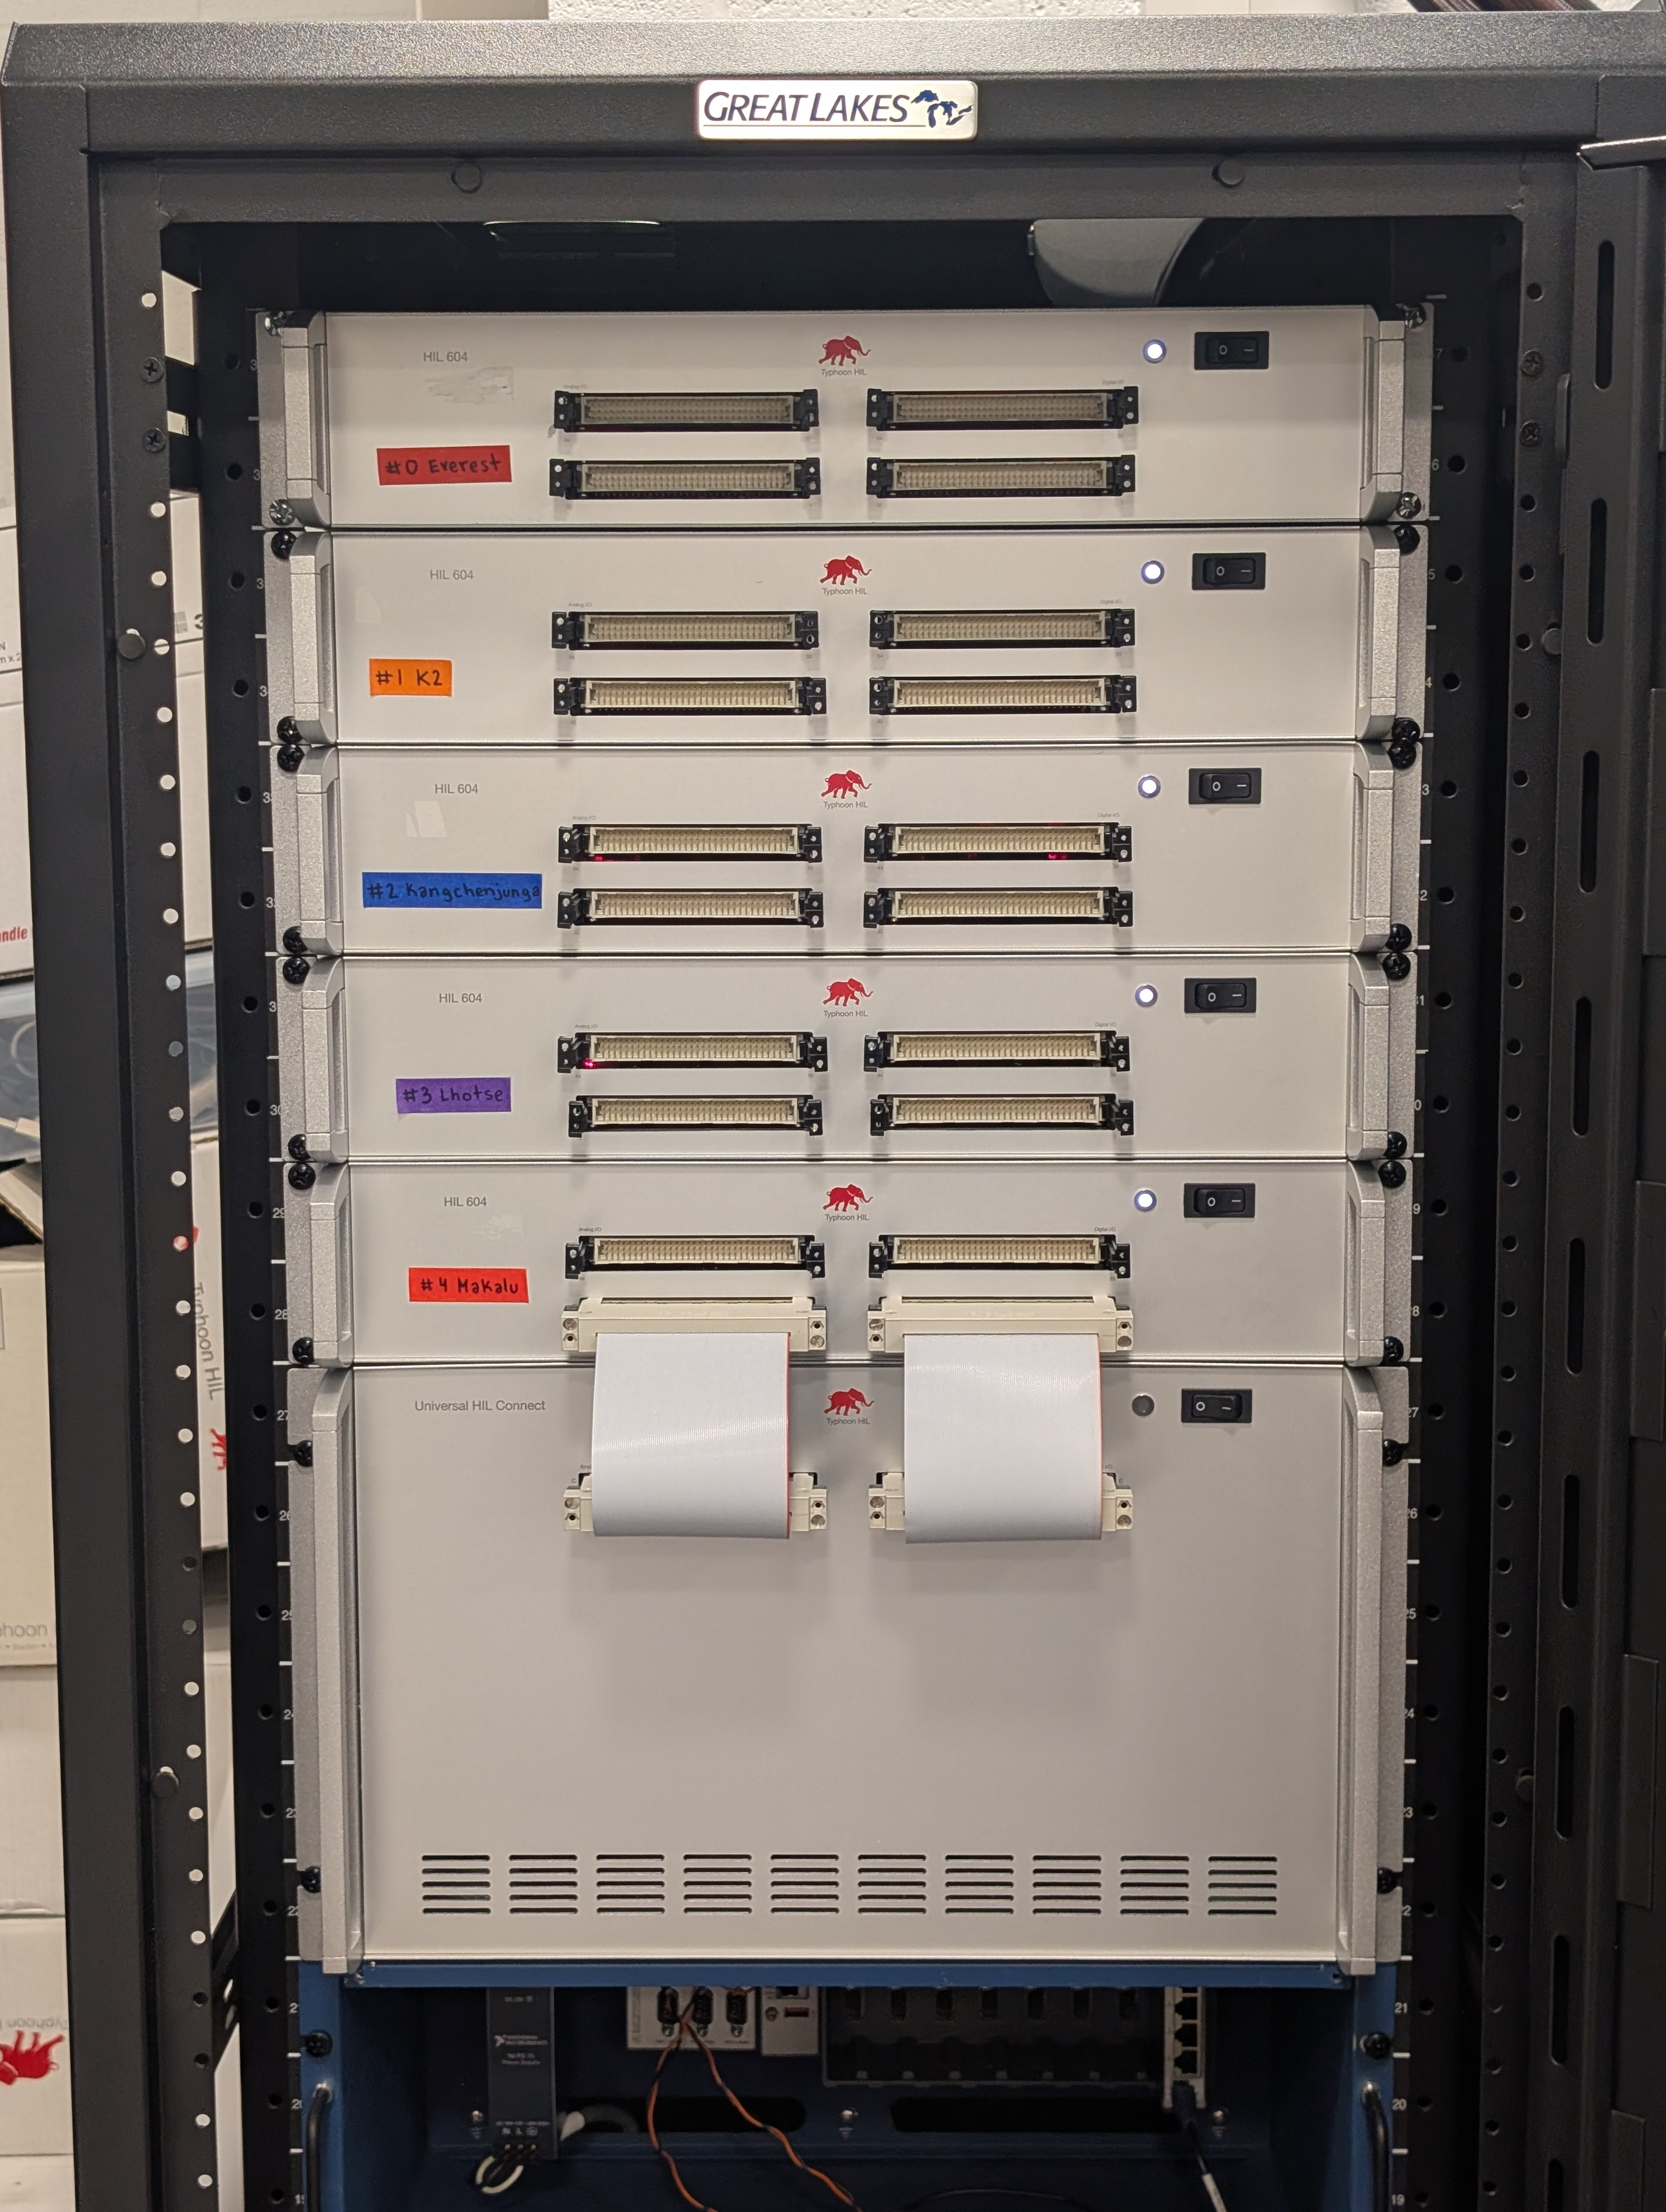
\includegraphics[height=0.6\textheight]{img/hils.jpg}
                \caption{Typhoon HIL 604 Simulators}
            \end{figure}
        \end{column}
    \end{columns}
\end{frame}

\begin{frame}
    \frametitle{Computational Hardware}
    \begin{columns}
        \begin{column}[T]{0.5\textwidth}
            \vspace{0pt}
            \begin{center}
                \textbf{Computational Nodes}
            \end{center}
            \begin{itemize}
                \item One Raspberry Pi 5, acting as a centralized controller
                \item Running Raspbian 12 (Bookworm)
                \item Adequate for our soft real-time requirements
            \end{itemize}
        \end{column}
        \begin{column}[T]{0.5\textwidth}
            \begin{figure}
                \includegraphics[height=0.6\textheight]{img/rpis.jpg}
                \caption{Small Cluster of Raspberry Pi's}
            \end{figure}
        \end{column}
    \end{columns}
\end{frame}

\begin{frame}
    \frametitle{BANSHEE Microgrid}
    \begin{figure}
        \includegraphics[width=\textwidth]{img/BANSHEE_Eric_side.pdf}
        \caption{BANSHEE: A prototypical Microgrid}
    \end{figure}
    % TODO add notes about BANSHEE!
    \note[]{}
\end{frame}

\begin{frame}
    \frametitle{Software}
    \begin{columns}
        \begin{column}[T]{0.4\textwidth}
            \vspace{0pt}
            \begin{itemize}
                \item Written in C++
                \item Uses Eigen for Linear Algebra
                \item Templated, both a static and dynamic allocation version
                \item Implements the \textbf{unconstrained} version of the algorithm
            \end{itemize}
        \end{column}
        \begin{column}[T]{0.6\textwidth}
            \vspace{-10pt}
            \begin{figure}
                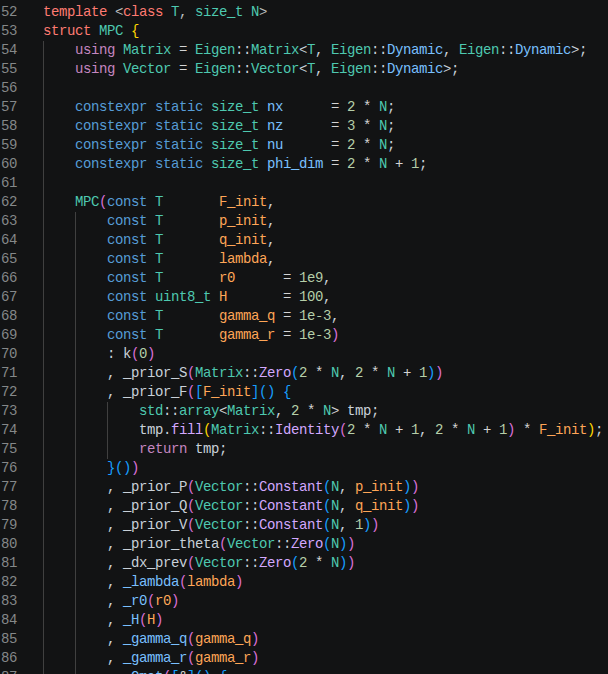
\includegraphics[height=0.65\textheight]{img/mpc_code_snippet.png}
                \caption{Snippet of the C++ Implementation}
            \end{figure}
        \end{column}
    \end{columns}
\end{frame}


\section{Numerical Results}
\begin{frame}
    \frametitle{The Scenario}
    \begin{columns}
        \begin{column}[T]{0.5\textwidth}
            \vspace{0pt}
            \begin{center}
                \textbf{Scenario}
            \end{center}
            \begin{itemize}
                \item Microgrid begins islanded from the bulk grid
                \item Initially 3.3MVA of load
                \item Over 8 seconds, 8 loads are manually enabled
                \item Final total load is 6.39MVA
                \item Controller runs the MPC loop every 10 milliseconds
            \end{itemize}
        \end{column}
        \begin{column}[T]{0.5\textwidth}
            \begin{center}
                \textbf{Desired Behavior}
            \end{center}
            \begin{itemize}
                \item As load increases, so to does generation
                \item Frequency may deviate temporarily, but returns to nominal
                \item Voltage may deviate temporarily, but returns to nominal
            \end{itemize}
        \end{column}
    \end{columns}
\end{frame}

\begin{frame}
    \frametitle{No Controller}
    \begin{figure}
        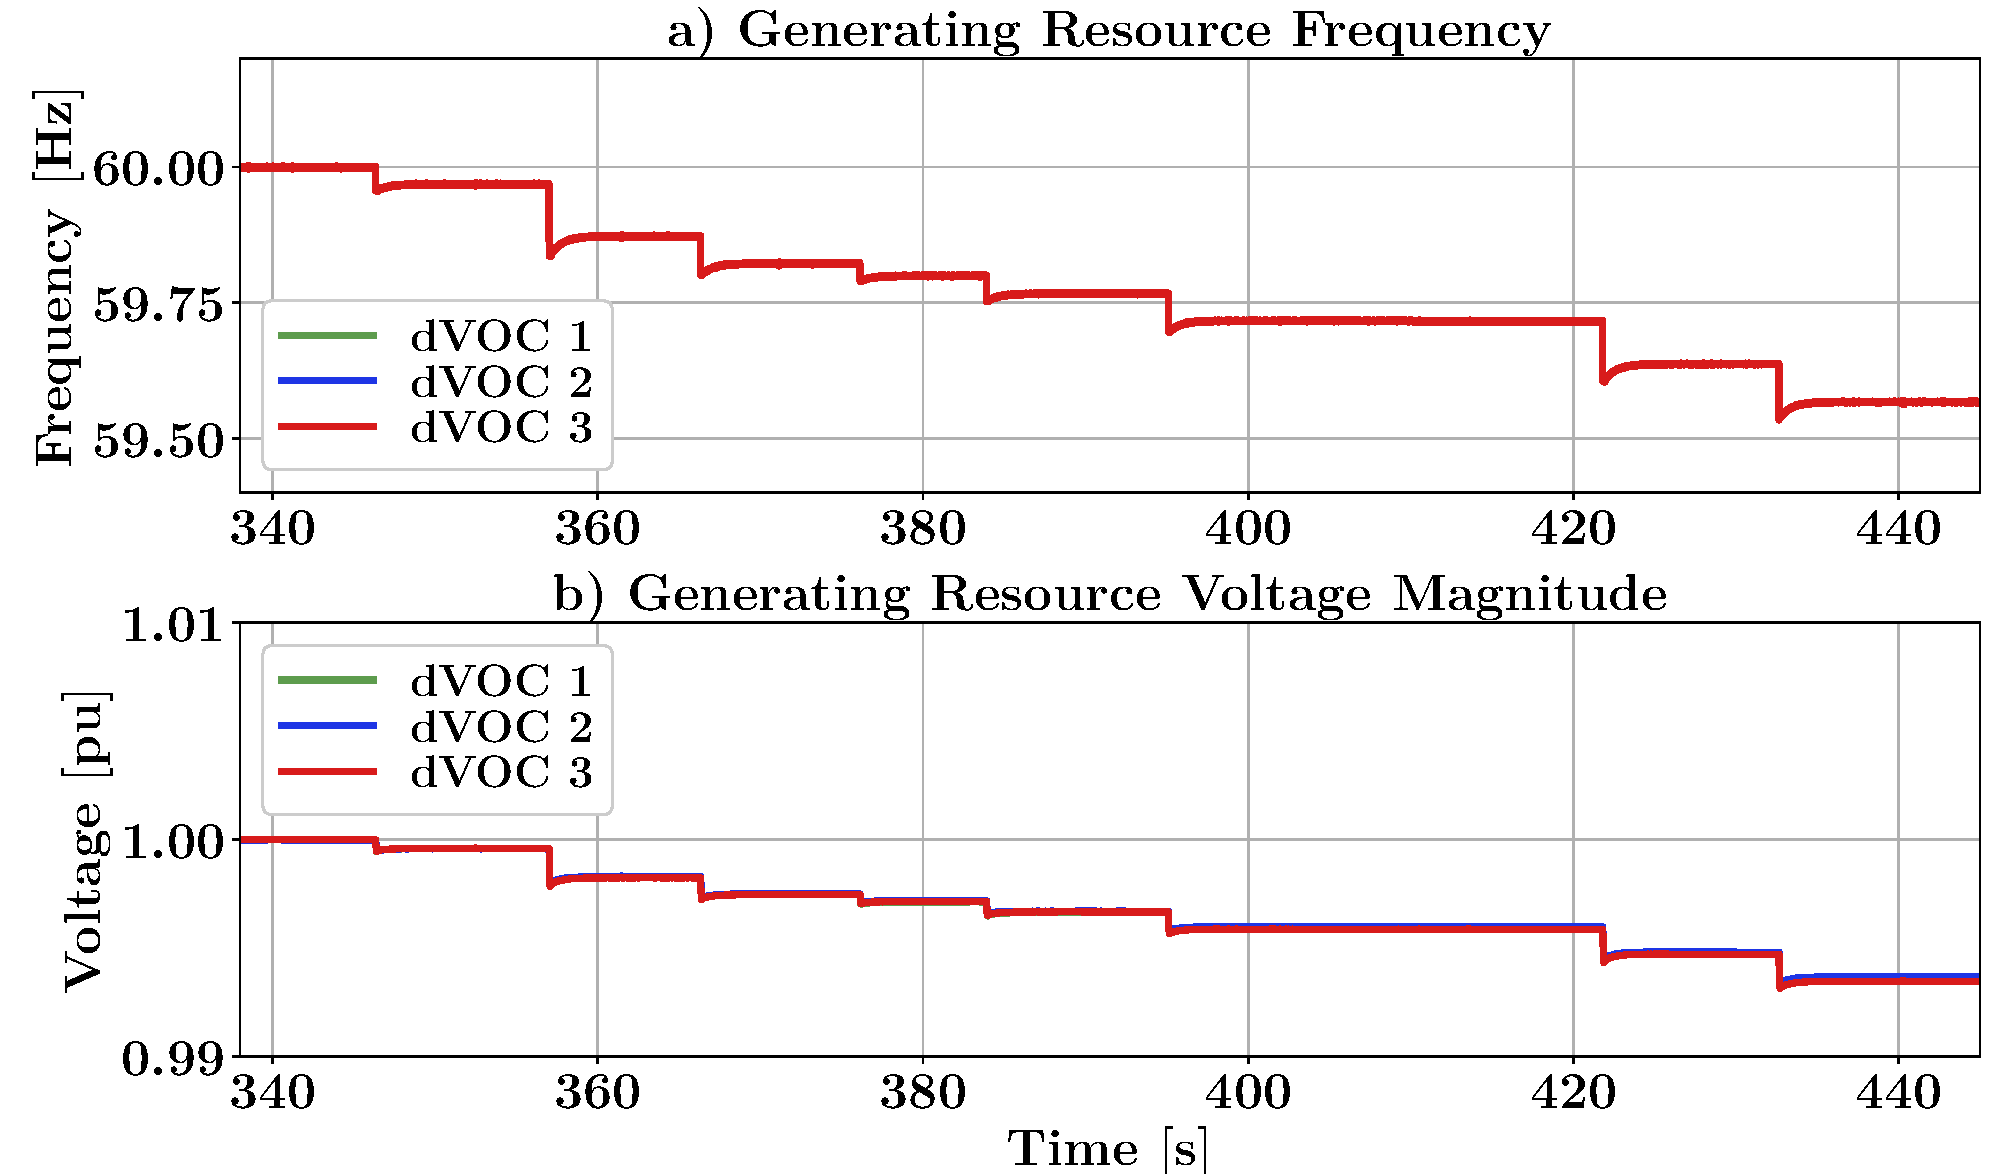
\includegraphics[height=0.7\textheight]{img/No_control_fv.pdf}
        \caption{Frequency and Voltage, no Controller}
    \end{figure}
\end{frame}
\begin{frame}
    \frametitle{Controller Enabled}
    \begin{figure}
        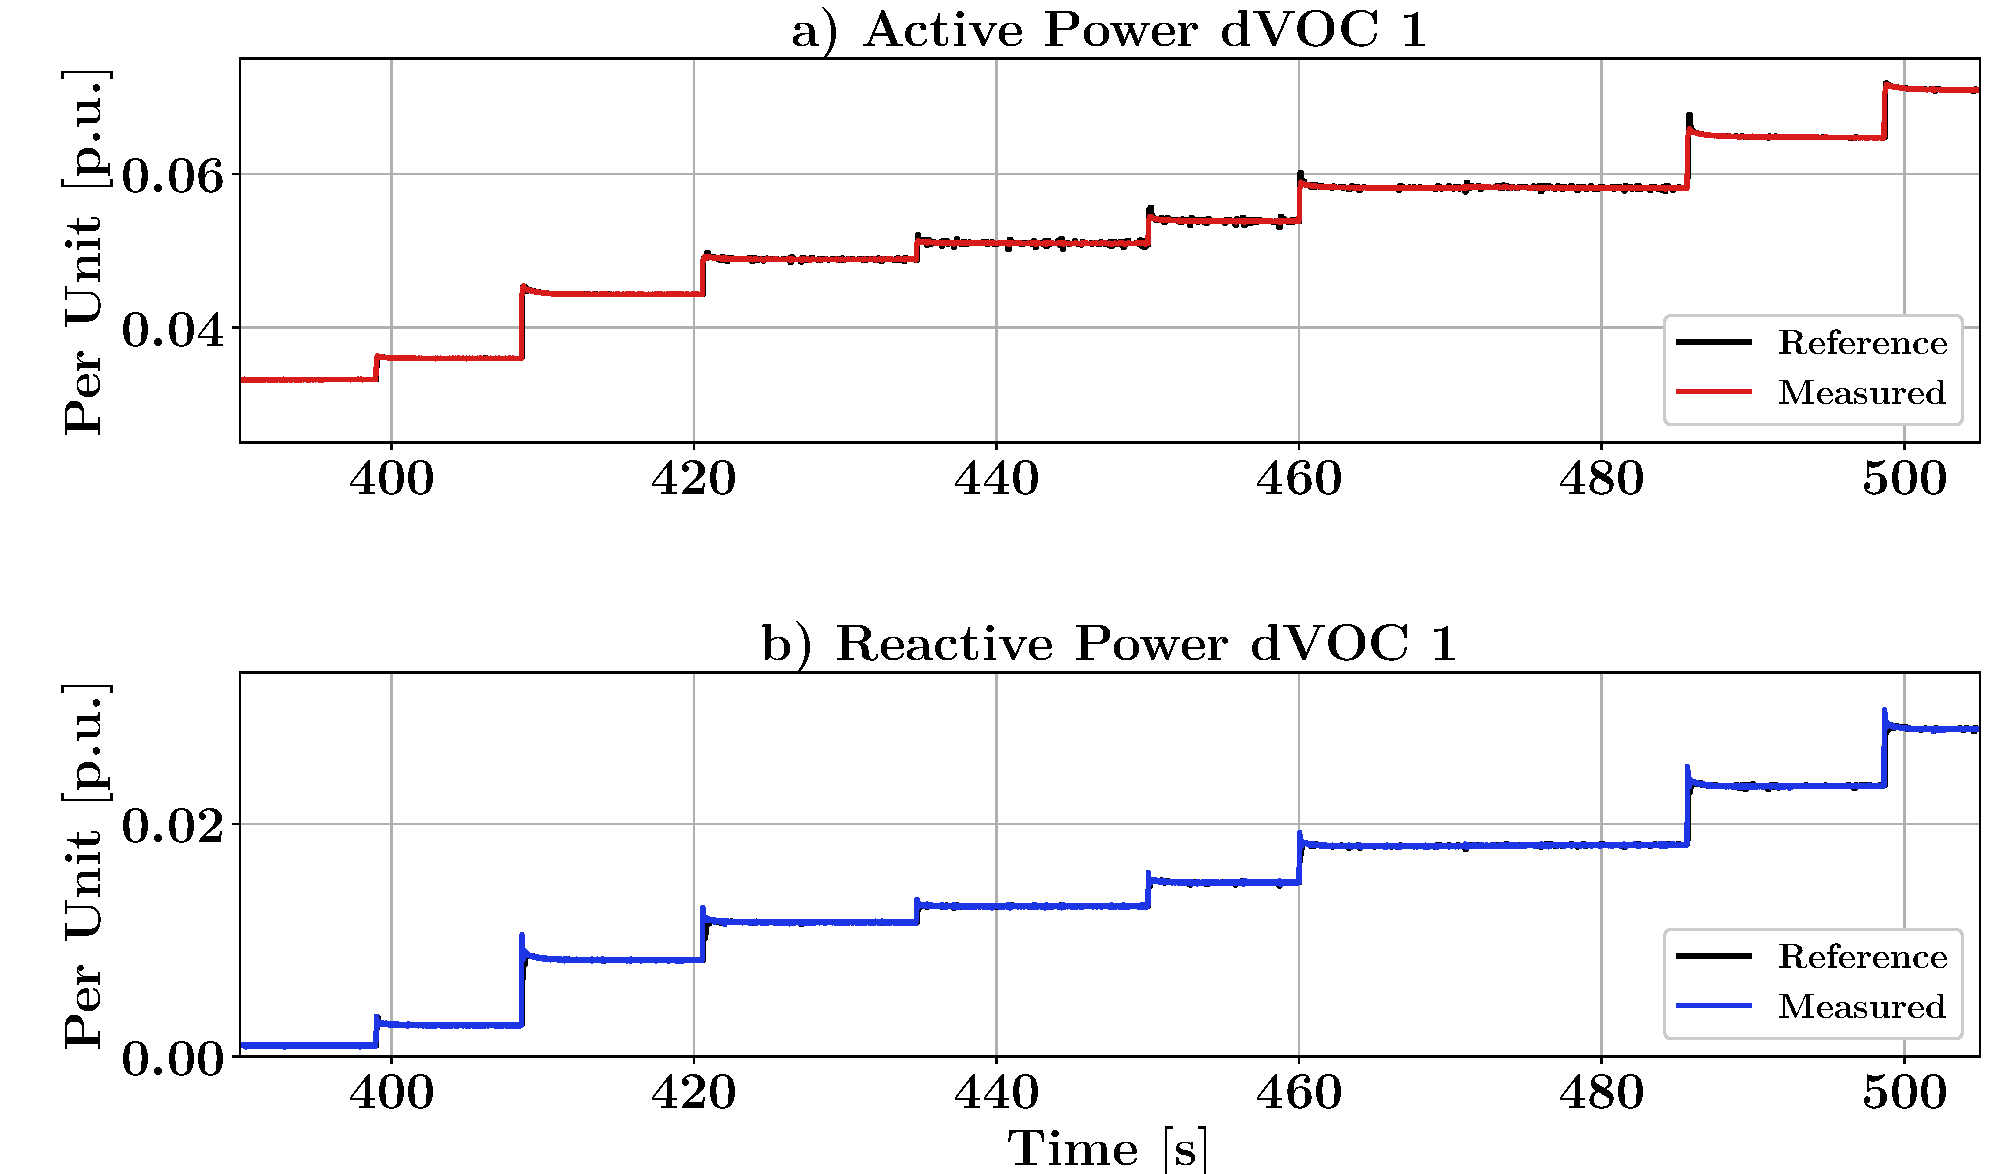
\includegraphics[height=0.7\textheight]{img/Control_pq.pdf}
        \caption{Active and Reactive Power Setpoints}
    \end{figure}
\end{frame}
\begin{frame}
    \frametitle{Controller Enabled}
    \begin{figure}
        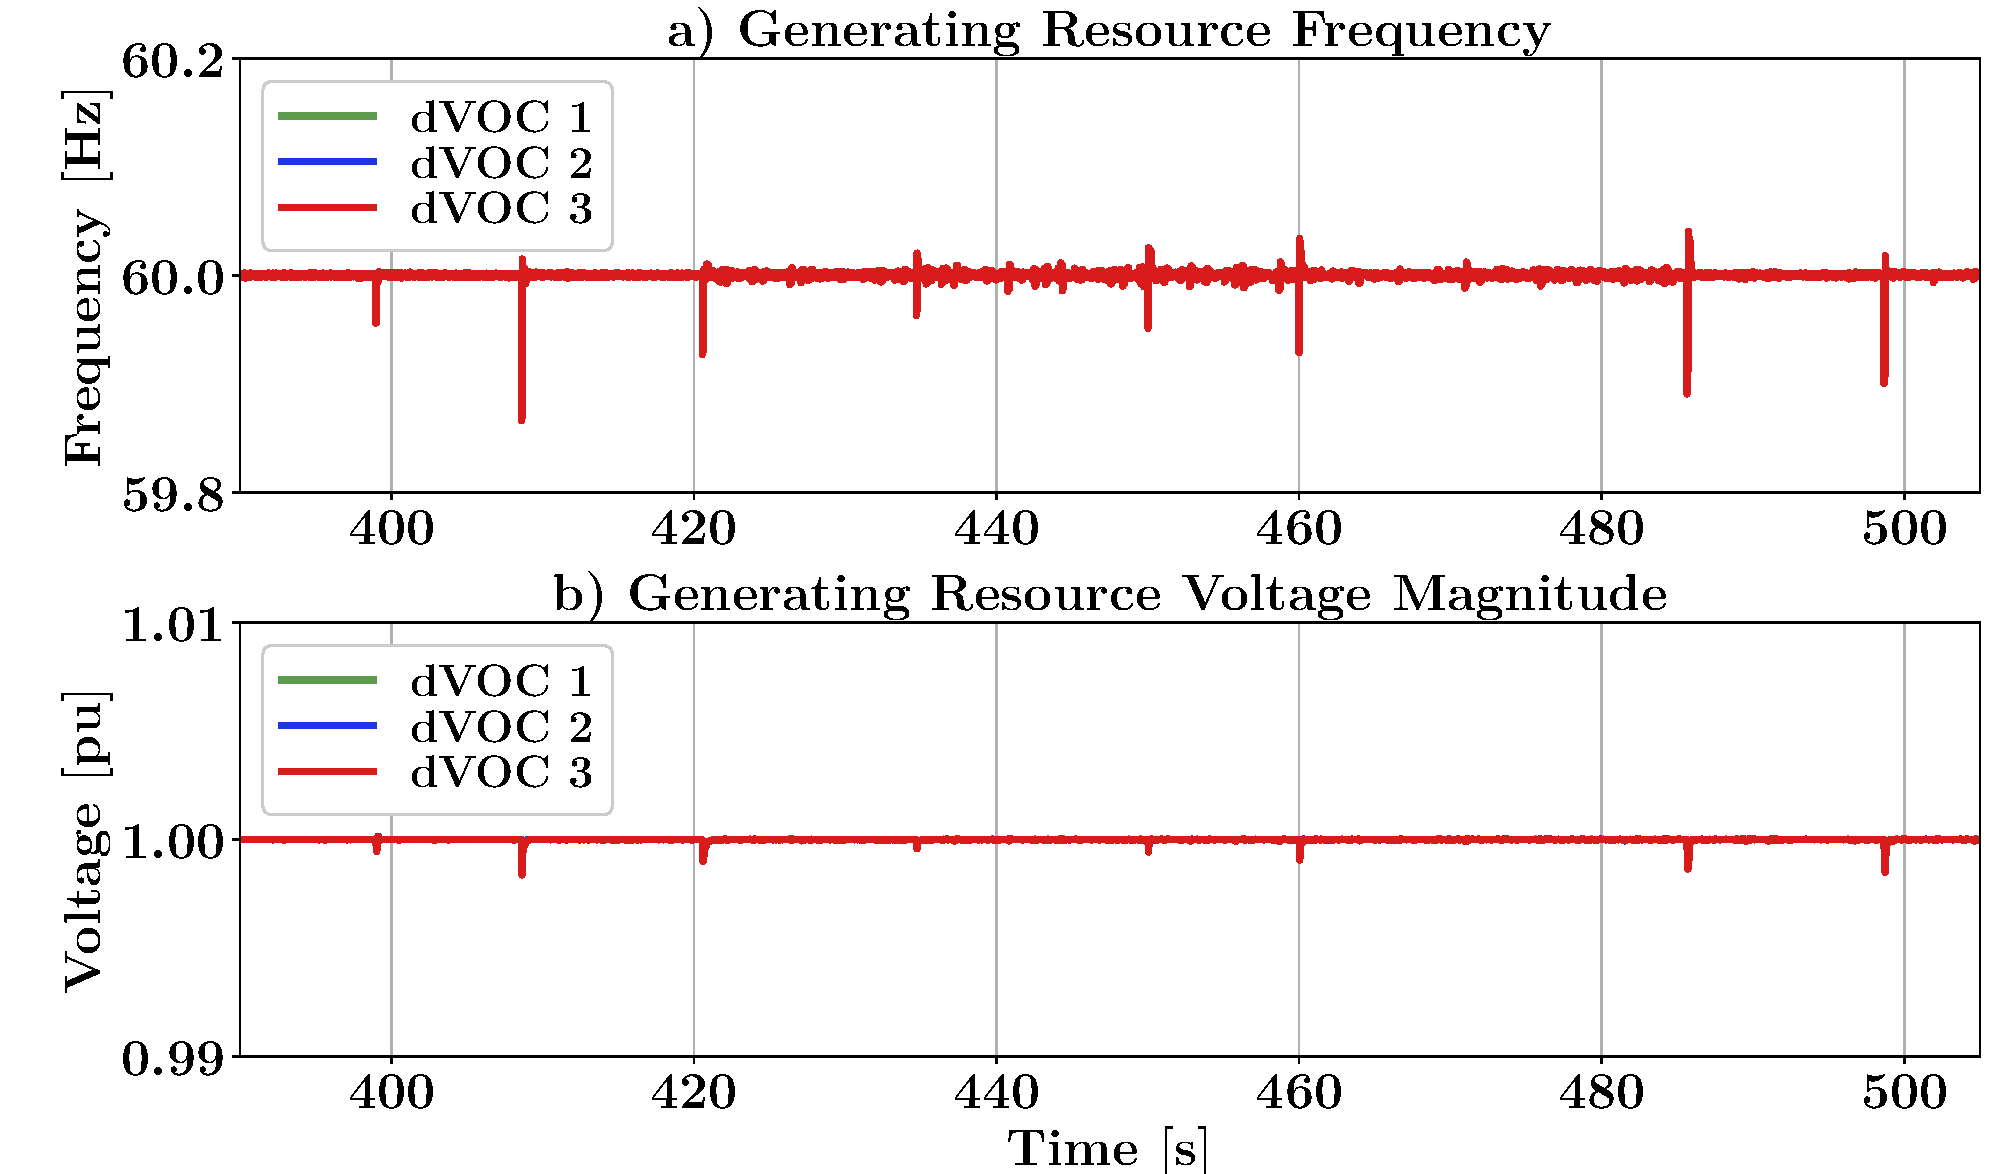
\includegraphics[height=0.7\textheight]{img/Control_fv.pdf}
        \caption{Frequency and Voltage, Controller Enabled}
    \end{figure}
\end{frame}

\section{Conclusion}
\begin{frame}
    \frametitle{Future Work}
    \begin{itemize}
        \item Implement constrained algorithm (in progress)
        \item Port to true real-time system
        \item Distributed version
        \item Test on varied systems
        \item Characterize performance
              \begin{itemize}
                  \item Algorithm
                  \item Software
              \end{itemize}
    \end{itemize}
\end{frame}

\begin{frame}
    \frametitle{Bibliography}
    \bibliographystyle{amsalpha}
    {
        \tiny
        \bibliography{qual_presentation.bib}
    }
\end{frame}
\begin{frame}
    \frametitle{Q\&A}
    \begin{center}
        \huge\textbf{Thank you!}
    \end{center}
\end{frame}
\end{document}